Assume that our current released version of software product is \texttt{v0.2.0} and there is a critical bug appears.
In order to release a hotfix the following set of steps to be executed:
\begin{enumerate}
    \item Hotfix to be assigned to a software engineer.
    \item Software engineer fixes critical bug and creates a pull request: \texttt{hotfix/id -> master}.
    Yes, pull request is done to the \texttt{master} branch.
    \item Pull request \texttt{hotfix/id -> master} is reviewed by team and merged.
    \item Release engineer cherry-picks~\cite{CherryPick} recently merged hotfix from the \texttt{master} branch
    to the \texttt{release/v0.2.0} branch.
    Note that branch \texttt{release/v0.2.0} is long-living and kept minimum until next release.
    \item Release engineer increments patch part of semantic version, e.g \texttt{v0.2.0 -> v0.2.1}.
    \item Release engineer creates and pushes new tag \texttt{v0.2.1}.
    \item Hotfix deployment process is started after new tag is pushed.
\end{enumerate}
\begin{figure}[H]
    \centering
    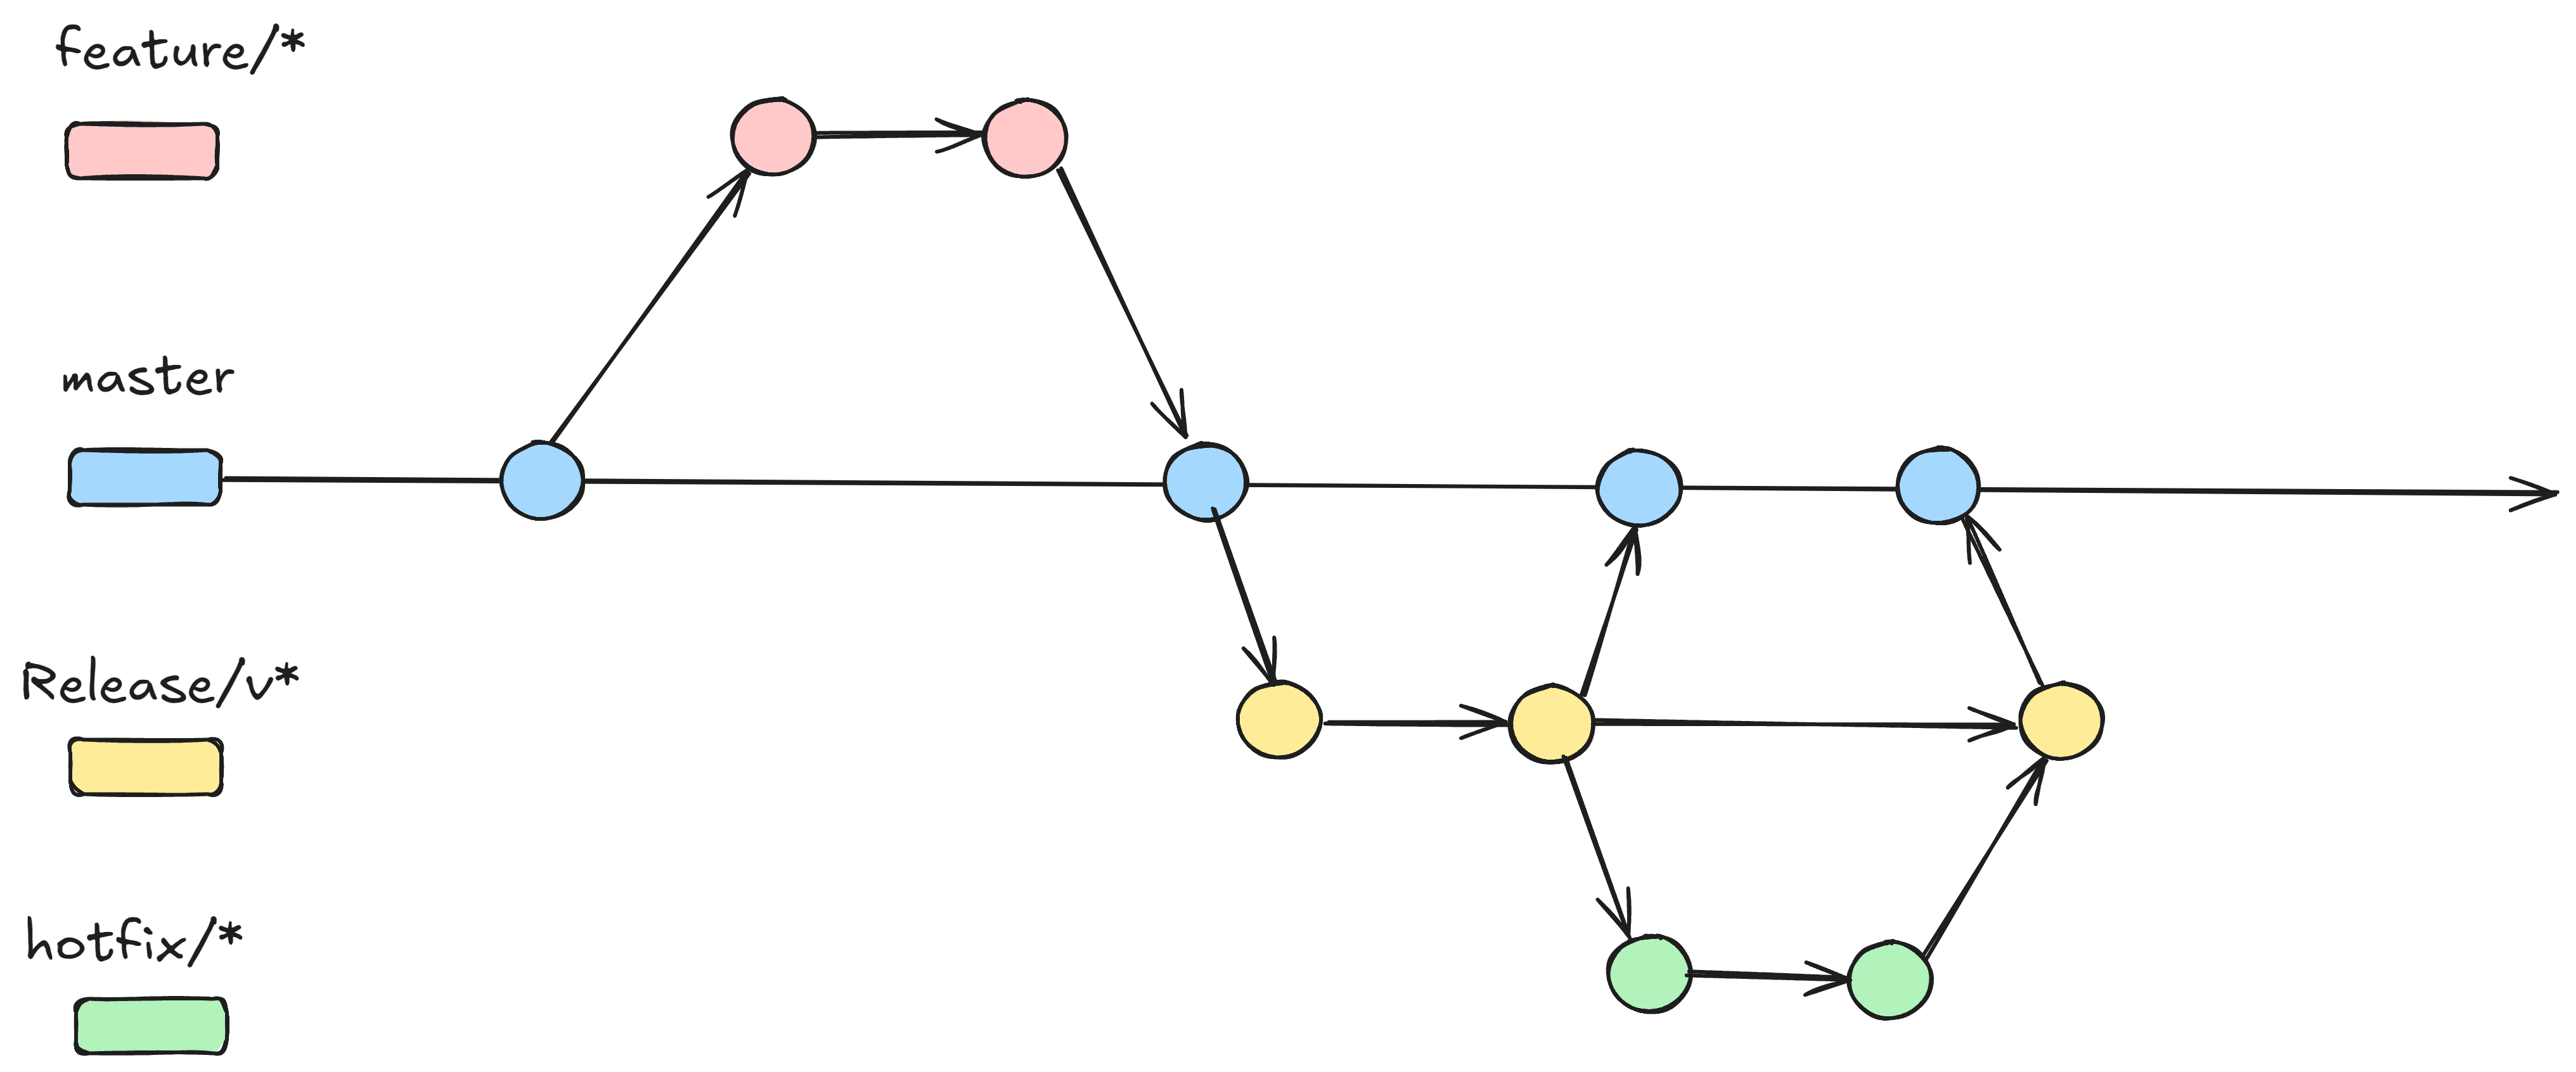
\includegraphics[width=1\textwidth]{img/HotFix_Strategy}
    ~\caption{Hotfix diagram.}\label{fig:hotfix-diagram}
\end{figure}

